\newgeometry{top=33mm,left=36mm,right=36mm,bottom=33mm,twoside,bindingoffset=8mm,headsep=1.8cm}
\pagestyle{empty}
\fancyhfoffset[E,O]{0pt}
\addtolength{\skip\footins}{\baselineskip}
{
\setlength{\parindent}{1.5em}

\hyphenation{polske-kompositörer}
\hyphenation{skaffare-mor}

%\setlength{\columnsep}{0.5cm}
%\vspace*{1cm}
%\begin{multicols}{2}
%\begin{adjustwidth*}{0mm}{0mm}
{\setlength{\parindent}{0mm}
Bland de många danser, som den gotländska befolkningen,
både gammal ock ung, med liv ock lust övade under den
tid, dansen ännu var populär hos den stora allmänheten, var
polskan den mäst omtyckta. Den var gotländingarnas hedersdans vid bröllop ock andra högtidliga tillfällen, den var deras huvuddans vid varjehanda andra glada samkväm, såsom vid »sletkalsgildar» (slåtteröl); vid »ating», då man samlades för att jälpa en släkting eller granne att täcka sitt ladugårdstak med den gotländska myragen; vid barndop, »bidningkalas»
(bjudningskalas), lekstugor ock andra tillfällen. Varhälst man dansade, var polskan oumbärlig. Under den tidrymd, polskan var så populär, gick nästan all folklig tondiktning ut på att skapa vackra polskemelodier. Vad de gamla bondspelmännen, ja stundom även mera musiklärda personer tänkte ock kände, gav sig under nämnda tid uttryck i dels glättiga, dels vemodsfulla melodier, men nästan alltid i \textemdash{} polsketakt. De svårare mollpolskemelodierna begagnades visserligen även på sina håll att dansa efter, men då deras innehåll ock skönhet förlorade på att föredragas i så raskt ock hurtigt tempo, som denna livliga dans kräver, spelades de på många ställen icke till
dans, utan endast »för att höra på». Durpolskemelodierna däremot utfördes mäst till dans ock föredrogos med skarpt markerad rytm.
}

\textit{Dansen} polska utfördes olika på olika ställen ock av olika åldrar, mäst parvis, men rätt ofta av flera par tillsammans.

I den s.\,k.\@ \textit{enkla} polskan, som utfördes av ett par, höllo de dansande antingen varandra i händerna, stundom med 
utsträckta, % står: utsträckta
stundom med böjda armar, eller ock höllo de med en hand vardera varandra om livet, ock de andra händerna höllos tillsammans något upplyftade med böjda armar. Svängningen skedde på senare tid alltid åt höger (»dansä ret»). Men i äldre tider (i slutet av 1700-talet) svängdes vid reprisombyte även åt vänster (»dansä avutt»), under det man i båda fallen trippade på tårna eller fotens främre del (börjande med högra foten) i takt med polskemelodiernas åttondelar. Svängningen skedde runt om, oavbrutet på samma ställe, där man började dansen. Det dansande par, som icke kunde hålla sig på samma plats (mitt i stugan), där de begynt dansen, utan vacklade än hit, än dit, stundom upp till spegeln, stundom ned till dörren, blev av det övriga sällskapet alldeles utskrattat.

De äldre, makliga gubbarna, orkade stundom ej trippa\footnote{»Trippa i åttondels takt», d.\,v.\,s.\@ man vrider sig på högra ock vänstra fotens främre delar ömsevis, i takt med polskans åttondelar.} åttondelarna, utan markerade endast fjärdedelarna (»ga u dansä»); men det oaktat kunde de med detta danssätt »sno» i så stark fart, att även den mäst danslystna flicka, som av dem fördes, kunde få trippa sig belåten. Vid lekstugor ock mindre högtidliga tillfällen utbytte ofta gossarna (karlarna) under en ock annan takt trippandet mot stampande (med hela fotsulan ock klacken), ävenledes då markerande åttondelarna.

På en del ställen brukade även glada gossar, sedan de bjudit upp en flicka, fatta hänne med högra armen om livet ock endast med denna arm »hålla fast» hänne, under det hans vänstra arm var fri ock utstående. På detta sätt svängde de ganska vidlyftigt omkring under de två första takterna av reprisen, därvid endast markerande fjärdedelarna. Därefter fattade de även med de hittils fria händerna om varandras liv ock snurrade raskt om, men »trippade» då alltid åttondelarna. Jag tror, att detta sätt att dansa icke får betraktas såsom något särskilt slag av polska. För min del anser jag detta fria svängande de två första takterna endast såsom en förberedelse eller inledning till den egentliga polskan, som gjorde det lättare att komma på takten (»kumm pa takti»), såsom de brukade säga.

Enligt gamla personers berättelser ock förevisningar, däribland
min farmor, som var född 1796 ock dog vid 84 års ålder, skulle man för hundra år sedan ock troligen ännu längre tillbaka i tiden, icke dansat polskan alldeles så, som jag här beskrivit, vilken beskrivning gäller för 1800-talet. Då markerades icke alla åttondelarna i takten, utan endast på första fjärdedelen trippades åttondelar, den första åttondelen med högra, den andra med vänstra foten (så som förut beskrivits); andra fjärdedelen markerades med högra foten, ock under det tredje fjärdedelen spelades i takten, hoppade man så att säga jämfota ett hopp med båda benen; samtidigt med detta hopp böjde man knäna mycket mera än i de två första fjärdedelarna åv varje takt. Under hela tiden svängdes åt höger, så länge en repris speltes, men vid reprisombyte
svängdes åt vänster med markering ock åtbörder på samma sätt, som då man dansade till vänster. Jag vill söka åskådliggöra, vad jag här sagt om de gamles sätt att dansa polska, genom att anföra de två första takterna av följande gamla polska med ord:

\vspace{0.6cm}
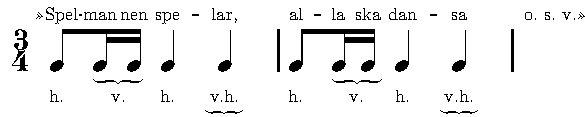
\includegraphics{include/snippets/spelmannen-spelar-crop.pdf}
\vspace{0.3cm}

Flera par kunde också tillsammans utföra denna dans (»dubbel polska»). Sedan ett par uppbjudit ett, två eller tre par till gemensam dans, bildade alla tillsammans en ring, som hölls ihop genom att man bjöd armarna åt de närmast stående, varefter t. ex. »gossarna» sammanflätade sina händer med de mitt emot stående »flickornas». Sedan alla nu förvissat sig om att de hade riktigt säkert tag, snurrade hela klungan om i rask fart på samma sätt, som beskrivet är om den enkla polskan.

I »disciplinerat» lag dansade aldrig mer än ett par i sänder, ock alltid i bestämd tur ock ordning. På senare tider urartade även denna sed, så att man kunde få se hela golvet fullt av dansande par, som samtidigt svängde dels parvis, dels i klungor (enkla ock dubbla polskan), så långt utrymmet medgav. Under de gamla spelmännens dagar hände det aldrig. Man höll sträng ock faderlig uppsikt över att allt måtte ordentligen tillgå.

Denna folkdans, så enkel ock föga omväxlande, kunde dock, där den utfördes med behag, liv ock lust, te sig ganska imponerande, i synnerhet vid ett ståtligare bondbröllop. Där börjades alltid dansen med minst tre, stundom fyra officiella skyldighetsdanser, vilka voro polskor. Den första var »skaffarepolskan», då skaffarefar ock skaffaremor, skaffaredrängen ock skaffarepigan måste dansa (eller ock lega för sig). Den andra hette »ungmansdrängspolskan», då dansade ungmansdrängarna ock brudpigorna (marskalkarna ock tärnorna). Den tredje hette »brudpolskan», då brudgummen ock bruden, bruttebonden ock bruttöverskan dansade med varandra. Den fjärde officiella polskan, som å vissa orter spelades, hette »kunämädrus» polska. Då skulle »kunämädru» (den närmaste ock mäst ansedda
kvinnliga släktingen i huset) dansa med närmaste ock mäst ansedda manliga släktingen i brudehuset. Huru det tillgick vid dessa danser, skildras av C. J. Bergman i »Gotländska skildringar och minnen» å s. 258-260 under rubriken »bondbröllop», i A. Th.\@ Snöboms »Gotlands land och folk» å s.\@ 339, 340 samt utförligast hos N. Lithberg i Fataburen 1911, s.\@ 153 if.

Om gotländska polskans \textit{ålder} kan jag icke bestämt upplysa. Vid flera tillfällen alltifrån barnaår hörde jag av framstående personer, att den har dansats här på ön ungefär tvåhundra år. Min nyss omnämnda farmor omtalade flera gånger för mig, att hännes farmor hade sjungit polskor ock dansat för hänne. Dessa polskor hade hon åter i sin ordning lärt av sina föräldrar ock så vidare. Men hur långt tillbaka i tiden
de spelats ock dansats här, kan jag ej bestämt säga. Visserligen påstod en gubbe i Hablingbo, att åtskilliga polskor, som han spelade, voro minst 250 år, men huruvida detta påstående äger grund, vill jag ej avgöra.

Angående polskans förekomst kan jag däremot bestämt säga, att den varit allmän överallt på ön, ifrån Fårö till Hoburgen, från östergarn till Västergarn. Många bevis finnas härpå. Ett säkert sådant är, att det finnes kända polskspelare ock polskekompositörer från alla delar av Gotland.

%%%%%%%%%%%%%%%%%%%%%%%%%%%%%%%%%%%%%%%%%%%%%%%%%%

\setlength{\parindent}{0mm}
\newpage

\subsection*{\centering Spelsätt.}
\vspace{5mm}

Om sättet, huru en del melodier spelades av de mäst framstående spelmännen.

\vspace{5mm}

\textit{Polskorna} voro under 1700- ock 1800-talen icke allenast spelmännens, utan även hela gotländska folkets favoritmelodier.

\vspace{5mm}

\textit{Durpolskorna} utfördes med liv ock lust i skarpt markerad takt ock med stark nyansering på första tonen i varje fjärdedel; med tonerna smidigt hopflätade ock sammanbundna (legato), så att flera takter understundom bildade liksom en kedja av toner, utan att stråken under tiden behövde lyftas från strängarna.

\vspace{5mm}

Exempel I.

\example{1}

\vspace{5mm}

Exempel II. Huru man spelade fyra säxtondelar i varje \guillemotright{}stråktag\guillemotright{}.

\example{2}

\vspace{10mm}

En typisk bild av starkt markerat ock bundet spel i polskan lämnas i nedanstående ex.
Detta spelsätt kallas på gotländska \textit{\guillemotright{}yverkast\guillemotright{}}
= överkast (kasta över).

\vspace{5mm}

Exempel III.

\example{3}

\newpage

Då man i säxtondels polskor skulle från en högre ton nå en eller flera lägre,
började man takten med uppstråk. Se nedanstående exempel IV ock V!

\vspace{5mm}

Exempel IV.

\example{4}

\vspace{5mm}

Exempel V.

\example{5}

Tonen \textit{d} i ovanstående exempel togs då alltid med 4:e fingret på bassträngen.

\vspace{10mm}

\textit{Mollpolskorna,} som ytterst sällan spelades till dans,
föredrogos i långsammare tempo ock markerades ej så skarpt
\textemdash{} spelades med allvar ock känsla. Dem skulle man blott
\guillemotright{}höra på\guillemotright{}.

\vspace{5mm}

Exempel VI.

\example{6}

\vspace{5mm}

Exempel VII.

\example{7}

\vspace{15mm}

\textit{Fler beskrivningar av spelsätt finns att läsa vid respektive låttyp.}


}
\restoregeometry
\fancyhfoffset[E,O]{0pt}
\clearpage
\pagestyle{main}
%\end{adjustwidth*}
%\end{multicols}
